%%%%%%%%%%%%%%%%%%%%%%%%%%%%%%%%%%%%%%%%%
% Jacobs Landscape Poster
% LaTeX Template
% Version 1.0 (29/03/13)
%
% Created by:
% Computational Physics and Biophysics Group, Jacobs University
% https://teamwork.jacobs-university.de:8443/confluence/display/CoPandBiG/LaTeX+Poster
% 
% Further modified by:
% Nathaniel Johnston (nathaniel@njohnston.ca)
%
% This template has been downloaded from:
% http://www.LaTeXTemplates.com
%
% License:
% CC BY-NC-SA 3.0 (http://creativecommons.org/licenses/by-nc-sa/3.0/)
%
%%%%%%%%%%%%%%%%%%%%%%%%%%%%%%%%%%%%%%%%%

%----------------------------------------------------------------------------------------
%	PACKAGES AND OTHER DOCUMENT CONFIGURATIONS
%----------------------------------------------------------------------------------------

\documentclass[final,20pt]{beamer}

\usepackage[scale=1.25]{beamerposter} % Use the beamerposter package for laying out the poster
\usepackage{amsmath}
\usepackage[makeroom]{cancel}
\usetheme{confposter} % Use the confposter theme supplied with this template

\setbeamercolor{block title}{fg=CMURed,bg=CMURed!20} % Colors of the block titles
\setbeamercolor{block body}{fg=black,bg=white} % Colors of the body of blocks
\setbeamercolor{block alerted title}{fg=white,bg=dblue!70} % Colors of the highlighted block titles
\setbeamercolor{block alerted body}{fg=black,bg=dblue!10} % Colors of the body of highlighted blocks
% Many more colors are available for use in beamerthemeconfposter.sty

%-----------------------------------------------------------
% Define the column widths and overall poster size
% To set effective sepwid, onecolwid and twocolwid values, first choose how many columns you want and how much separation you want between columns
% In this template, the separation width chosen is 0.024 of the paper width and a 4-column layout
% onecolwid should therefore be (1-(# of columns+1)*sepwid)/# of columns e.g. (1-(4+1)*0.024)/4 = 0.22
% Set twocolwid to be (2*onecolwid)+sepwid = 0.464
% Set threecolwid to be (3*onecolwid)+2*sepwid = 0.708

\newlength{\sepwid}
\newlength{\onecolwid}
\newlength{\twocolwid}
\newlength{\threecolwid}
\setlength{\paperwidth}{48.0in} % A0 width: 46.8in
\setlength{\paperheight}{36in} % A0 height: 33.1in
\setlength{\sepwid}{0.020\paperwidth} % Separation width (white space) between columns
\setlength{\onecolwid}{0.30\paperwidth} % Width of one column
\setlength{\twocolwid}{0.6\paperwidth} % Width of two columns
\setlength{\threecolwid}{0.9\paperwidth} % Width of three columns
\setlength{\topmargin}{1.2in} % Reduce the top margin size
%-----------------------------------------------------------
\usepackage{booktabs} % Top and bottom rules for tables
\usepackage{verbatim}
\usepackage{graphicx}
\usepackage{amsmath, amssymb, amsthm}
\usepackage{mathtools}
\usepackage{tabularx}
\usepackage{etex}
\usepackage{exscale}
\usepackage{multirow}
\usepackage{multicol}
\usepackage{mathtools}
\usepackage{fancyvrb}
\usepackage{algorithm}
\usepackage{algpseudocode}
\usepackage{float}
\usepackage{listings}
\usepackage{algorithm}
\usepackage{algorithmic}
\usepackage{times}
\usepackage{subfigure}

\usepackage{wrapfig}


%%%%%%%%%%%%%%%%%%%%%%%%%%%%%%%%%%%%%%%%%%
% Custom commands                        %
%%%%%%%%%%%%%%%%%%%%%%%%%%%%%%%%%%%%%%%%%%

\newcommand{\vc}[1]{\boldsymbol{#1}}
\newcommand{\adj}[1]{\frac{d J}{d #1}}
\newcommand{\chain}[2]{\adj{#2} = \adj{#1}\frac{d #1}{d #2}}
\newcommand\norm[1]{\left\lVert#1\right\rVert}

% mathcal
\newcommand{\Ac}{\mathcal{A}}
\newcommand{\Bc}{\mathcal{B}}
\newcommand{\Cc}{\mathcal{C}}
\newcommand{\Dc}{\mathcal{D}}
\newcommand{\Ec}{\mathcal{E}}
\newcommand{\Fc}{\mathcal{F}}
\newcommand{\Gc}{\mathcal{G}}
\newcommand{\Hc}{\mathcal{H}}
\newcommand{\Ic}{\mathcal{I}}
\newcommand{\Jc}{\mathcal{J}}
\newcommand{\Kc}{\mathcal{K}}
\newcommand{\Lc}{\mathcal{L}}
\newcommand{\Mc}{\mathcal{M}}
\newcommand{\Nc}{\mathcal{N}}
\newcommand{\Oc}{\mathcal{O}}
\newcommand{\Pc}{\mathcal{P}}
\newcommand{\Qc}{\mathcal{Q}}
\newcommand{\Rc}{\mathcal{R}}
\newcommand{\Sc}{\mathcal{S}}
\newcommand{\Tc}{\mathcal{T}}
\newcommand{\Uc}{\mathcal{U}}
\newcommand{\Vc}{\mathcal{V}}
\newcommand{\Wc}{\mathcal{W}}
\newcommand{\Xc}{\mathcal{X}}
\newcommand{\Yc}{\mathcal{Y}}
\newcommand{\Zc}{\mathcal{Z}}

% mathbb
\newcommand{\Ab}{\mathbb{A}}
\newcommand{\Bb}{\mathbb{B}}
\newcommand{\Cb}{\mathbb{C}}
\newcommand{\Db}{\mathbb{D}}
\newcommand{\Eb}{\mathbb{E}}
\newcommand{\Fb}{\mathbb{F}}
\newcommand{\Gb}{\mathbb{G}}
\newcommand{\Hb}{\mathbb{H}}
\newcommand{\Ib}{\mathbb{I}}
\newcommand{\Jb}{\mathbb{J}}
\newcommand{\Kb}{\mathbb{K}}
\newcommand{\Lb}{\mathbb{L}}
\newcommand{\Mb}{\mathbb{M}}
\newcommand{\Nb}{\mathbb{N}}
\newcommand{\Ob}{\mathbb{O}}
\newcommand{\Pb}{\mathbb{P}}
\newcommand{\Qb}{\mathbb{Q}}
\newcommand{\Rb}{\mathbb{R}}
\newcommand{\Sb}{\mathbb{S}}
\newcommand{\Tb}{\mathbb{T}}
\newcommand{\Ub}{\mathbb{U}}
\newcommand{\Vb}{\mathbb{V}}
\newcommand{\Wb}{\mathbb{W}}
\newcommand{\Xb}{\mathbb{X}}
\newcommand{\Yb}{\mathbb{Y}}
\newcommand{\Zb}{\mathbb{Z}}

% mathbf lowercase
\newcommand{\av}{\mathbf{a}}
\newcommand{\bv}{\mathbf{b}}
\newcommand{\cv}{\mathbf{c}}
\newcommand{\dv}{\mathbf{d}}
\newcommand{\ev}{\mathbf{e}}
\newcommand{\fv}{\mathbf{f}}
\newcommand{\gv}{\mathbf{g}}
\newcommand{\hv}{\mathbf{h}}
\newcommand{\iv}{\mathbf{i}}
\newcommand{\jv}{\mathbf{j}}
\newcommand{\kv}{\mathbf{k}}
\newcommand{\lv}{\mathbf{l}}
\newcommand{\mv}{\mathbf{m}}
\newcommand{\nv}{\mathbf{n}}
\newcommand{\ov}{\mathbf{o}}
\newcommand{\pv}{\mathbf{p}}
\newcommand{\qv}{\mathbf{q}}
\newcommand{\rv}{\mathbf{r}}
\newcommand{\sv}{\mathbf{s}}
\newcommand{\tv}{\mathbf{t}}
\newcommand{\uv}{\mathbf{u}}
\newcommand{\vv}{\mathbf{v}}
\newcommand{\wv}{\mathbf{w}}
\newcommand{\xv}{\mathbf{x}}
\newcommand{\yv}{\mathbf{y}}
\newcommand{\zv}{\mathbf{z}}

% mathbf uppercase
\newcommand{\Av}{\mathbf{A}}
\newcommand{\Bv}{\mathbf{B}}
\newcommand{\Cv}{\mathbf{C}}
\newcommand{\Dv}{\mathbf{D}}
\newcommand{\Ev}{\mathbf{E}}
\newcommand{\Fv}{\mathbf{F}}
\newcommand{\Gv}{\mathbf{G}}
\newcommand{\Hv}{\mathbf{H}}
\newcommand{\Iv}{\mathbf{I}}
\newcommand{\Jv}{\mathbf{J}}
\newcommand{\Kv}{\mathbf{K}}
\newcommand{\Lv}{\mathbf{L}}
\newcommand{\Mv}{\mathbf{M}}
\newcommand{\Nv}{\mathbf{N}}
\newcommand{\Ov}{\mathbf{O}}
\newcommand{\Pv}{\mathbf{P}}
\newcommand{\Qv}{\mathbf{Q}}
\newcommand{\Rv}{\mathbf{R}}
\newcommand{\Sv}{\mathbf{S}}
\newcommand{\Tv}{\mathbf{T}}
\newcommand{\Uv}{\mathbf{U}}
\newcommand{\Vv}{\mathbf{V}}
\newcommand{\Wv}{\mathbf{W}}
\newcommand{\Xv}{\mathbf{X}}
\newcommand{\Yv}{\mathbf{Y}}
\newcommand{\Zv}{\mathbf{Z}}

% bold greek lowercase
\newcommand{\alphav     }{\boldsymbol \alpha     }
\newcommand{\betav      }{\boldsymbol \beta      }
\newcommand{\gammav     }{\boldsymbol \gamma     }
\newcommand{\deltav     }{\boldsymbol \delta     }
\newcommand{\epsilonv   }{\boldsymbol \epsilon   }
\newcommand{\varepsilonv}{\boldsymbol \varepsilon}
\newcommand{\zetav      }{\boldsymbol \zeta      }
\newcommand{\etav       }{\boldsymbol \eta       }
\newcommand{\thetav     }{\boldsymbol \theta     }
\newcommand{\varthetav  }{\boldsymbol \vartheta  }
\newcommand{\iotav      }{\boldsymbol \iota      }
\newcommand{\kappav     }{\boldsymbol \kappa     }
\newcommand{\varkappav  }{\boldsymbol \varkappa  }
\newcommand{\lambdav    }{\boldsymbol \lambda    }
\newcommand{\muv        }{\boldsymbol \mu        }
\newcommand{\nuv        }{\boldsymbol \nu        }
\newcommand{\xiv        }{\boldsymbol \xi        }
\newcommand{\omicronv   }{\boldsymbol \omicron   }
\newcommand{\piv        }{\boldsymbol \pi        }
\newcommand{\varpiv     }{\boldsymbol \varpi     }
\newcommand{\rhov       }{\boldsymbol \rho       }
\newcommand{\varrhov    }{\boldsymbol \varrho    }
\newcommand{\sigmav     }{\boldsymbol \sigma     }
\newcommand{\varsigmav  }{\boldsymbol \varsigma  }
\newcommand{\tauv       }{\boldsymbol \tau       }
\newcommand{\upsilonv   }{\boldsymbol \upsilon   }
\newcommand{\phiv       }{\boldsymbol \phi       }
\newcommand{\varphiv    }{\boldsymbol \varphi    }
\newcommand{\chiv       }{\boldsymbol \chi       }
\newcommand{\psiv       }{\boldsymbol \psi       }
\newcommand{\omegav     }{\boldsymbol \omega     }

% bold greek uppercase
\newcommand{\Gammav     }{\boldsymbol \Gamma     }
\newcommand{\Deltav     }{\boldsymbol \Delta     }
\newcommand{\Thetav     }{\boldsymbol \Theta     }
\newcommand{\Lambdav    }{\boldsymbol \Lambda    }
\newcommand{\Xiv        }{\boldsymbol \Xi        }
\newcommand{\Piv        }{\boldsymbol \Pi        }
\newcommand{\Sigmav     }{\boldsymbol \Sigma     }
\newcommand{\Upsilonv   }{\boldsymbol \Upsilon   }
\newcommand{\Phiv       }{\boldsymbol \Phi       }
\newcommand{\Psiv       }{\boldsymbol \Psi       }
\newcommand{\Omegav     }{\boldsymbol \Omega     }


\setbeamerfont{itemize/enumerate subbody}{size=\normalsize} %to set the body size
\setbeamertemplate{itemize subitem}{\normalsize\raise1.25pt\hbox{\donotcoloroutermaths$\blacktriangleright$}}  %to set the symbol size
%\floatname{algorithm}{Procedure}
\renewcommand{\algorithmicrequire}{\textbf{Input:}}
\renewcommand{\algorithmicensure}{\textbf{Output:}}
\newcommand{\abs}[1]{\lvert#1\rvert}
\newcommand{\norm}[1]{\lVert#1\rVert}
\newcommand{\RR}{\mathbb{R}}
\newcommand{\CC}{\mathbb{C}}
\newcommand{\Nat}{\mathbb{N}}
\newcommand{\br}[1]{\{#1\}}
\renewcommand{\lstlistingname}{Code}
\DeclareMathOperator*{\argmin}{arg\,min}
\DeclareMathOperator*{\argmax}{arg\,max}

% Add the Logo Of CMU to the title
\setbeamertemplate{headline}{
 \leavevmode
  \begin{columns}
   \begin{column}{.1\linewidth}
    
\includegraphics[width=0.9\linewidth]{CMUlogo.png}
   \end{column}
   \begin{column}{.6\linewidth}
    \centering
    \usebeamercolor{title in headline}{\color{CMURed}\Huge{\textbf{\inserttitle}}\\[0.5ex]}
    \usebeamercolor{author in headline}{\color{fg}\Large{\insertauthor}\\[0.2ex]}
    \usebeamercolor{institute in headline}{\color{fg}\Large{\insertinstitute}\\[0.5ex]}
    \vskip1cm
   \end{column}
   \begin{column}{.15\linewidth}
    % \includegraphics[width=1.0\linewidth]{mllogo.jpg}
    
\includegraphics[width=1.2\linewidth]{ltilogo.png}
   \end{column}
  \end{columns}
 \hspace{0.5in}\begin{beamercolorbox}[wd=47in,colsep=0.15cm]{cboxb}\end{beamercolorbox}
}

%----------------------------------------------------------------------------------------
%	TITLE SECTION 
%----------------------------------------------------------------------------------------

\title{Label-Aware Attention for Fine-Grained Emotion Detection}
\author{Yilin Wang, Ethan Wu, Ziqi Liu \\
\{yilinwan, yongyiw, ziqil2\}@andrew.cmu.edu}
\institute{Carnegie Mellon University} 

%----------------------------------------------------------------------------------------

%% document start from here
\begin{document}

\addtobeamertemplate{block end}{}{\vspace*{1ex}} % White space under blocks
\addtobeamertemplate{block alerted end}{}{\vspace*{1ex}} % White space under highlighted (alert) blocks

\setlength{\belowcaptionskip}{1ex} % White space under figures
\setlength\belowdisplayshortskip{1ex} % White space under equations

\begin{frame}[t] % The whole poster is enclosed in one beamer frame

\begin{columns}[t] % The whole poster consists of three major columns, the second of which is split into two columns twice - the [t] option aligns each column's content to the top







%%%%%%%%%%%%%%%%%%%%%%%%%%%%%%%%%%%%%%%%%edit from here


%%%%%%%%%%%%% place a spacer between columns:
\begin{column}{\sepwid}\end{column} % Empty spacer column

%%%%%%%%%%%%% start your columns by doing this:

\begin{column}{\onecolwid} % The first column

%%%%%%%%%%%%%


\vspace*{-0.5in}

%%%%%%%%%%%%%%%%% begin section by doing this:
\begin{block}{Introduction}


%%%%%%%%%%%%%%%%%% begin subsection by doing this
% \textcolor{CMURed}{\textbf{FILL HERE WITH SUBSECTION}:}

%%%%%%%%%%%%%%%%%% begin your text by writing in subsection:
As an active NLP domain, emotion detection aims to determine the emotion(s) behind the plain text. GoEmotions dataset presents a multi-label classification challenge with more fine-grained emotion taxonomy than previous benchmarks. We propose a label-aware attention mechanism which significantly outperforms the baseline model. 

%%%%%%%%%%%%%%%%%% end your section here by doing this:::
\end{block}


%%%%%%%%%%%%%%%%%% begin second section in the same column:
\begin{block}{Task}
GoEmotions consists of 58K English Reddit comments, each labelled with one or more of the 28 emotions, including neutral. The baseline classifier proposed by the author is trained by finetuning a BERT model on this dataset, which yields the macro F1-score 0.46. 

\begin{columns}
\begin{column}{0.5\linewidth}
\begin{figure}
    \centering
    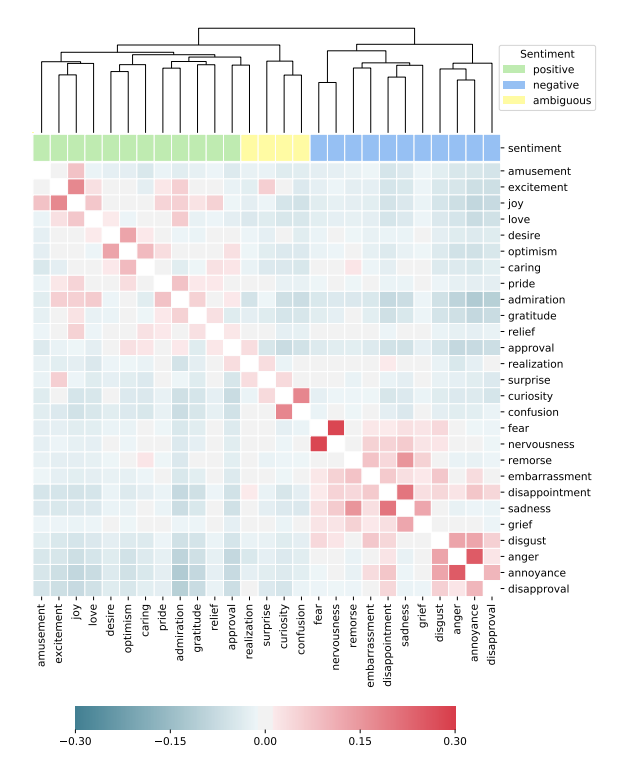
\includegraphics[width=20cm]{corr.png}
    \caption{Label correlation}
    \label{fig:corr}
\end{figure}
\end{column}
~
\begin{column}{0.4\linewidth}
\begin{table}
    \centering
    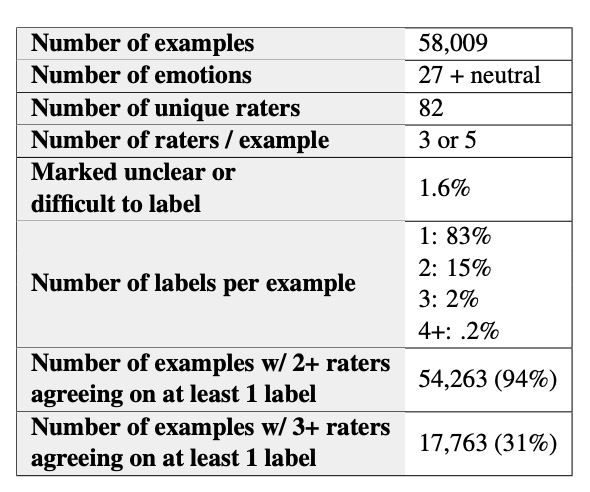
\includegraphics[width=15cm]{stat.png}
    \caption{Statistics of the GoEmotions dataset. We see that 83\% of the samples have single label, and class ``neutral" makes up 26\% of all samples.}
    \label{fig:my_label}
\end{table}
\end{column}
\end{columns}
\vspace{1ex}
% One way to improve performance would be to facilitate natural language understanding (NLU). In this particular task, the labels (emotions) carry some meaning. In addition, emotions are correlated to each other, as shown in Figure \ref{fig:corr}. One way to improve the NLU is to incorporate label semantics in the construction of the model. This idea motivated our improvement upon the baseline model.  

The challenge of the GoEmotions dataset comes from its fine-grained taxonomy. As illustrated in Figure \ref{fig:corr}, many emotions are in fact semantically and statistically correlated. After performing error analysis on the baseline model, we found that ``neutral" is often confused with other emotions, and low-resourced emotions are often misclassified as high-resourced ones with similar sentiment. 

% We realized that the model may not understand the meaning of the texts, but it relied on some patterns of the sentence to make the classification. 


%%%%%%%%%%%%%%%%%% end second section in the same column:
\end{block}



%%%%%%%%%%%%%%%%%% end your column:
\end{column} % End of the first column

%%%%%%%%%%%%%%%%%% Put a spacer between columns
\begin{column}{\sepwid}\end{column} % Empty spacer column

%%%%%%%%%%%%%%%%%% start second column:
\begin{column}{\onecolwid} 
\vspace*{-0.5in}
\begin{block}{Method}
To mitigate the naively assumed independence between emotions (labels), we introduce an label-aware attention mechanism, where each emotion is enabled to focus on different aspects of a sentence, depending on the semantic representation of the emotion label. 

\begin{figure}
\begin{center}
    \tikzset{every picture/.style={line width=0.75pt}} %set default line width to 0.75pt

\begin{tikzpicture}[x=0.75pt,y=0.75pt,yscale=-2.5,xscale=2.5]
%uncomment if require: \path (0,440); %set diagram left start at 0, and has height of 440

%Straight Lines [id:da31370839057744115] 
\draw [color={rgb, 255:red, 0; green, 0; blue, 0 }  ,draw opacity=0.25 ]   (347.15,213.51) -- (396.86,163.08) ;
\draw [shift={(398.96,160.94)}, rotate = 134.59] [fill={rgb, 255:red, 0; green, 0; blue, 0 }  ,fill opacity=0.25 ][line width=0.08]  [draw opacity=0] (3.57,-1.72) -- (0,0) -- (3.57,1.72) -- cycle    ;
%Straight Lines [id:da20644252238970973] 
\draw [color={rgb, 255:red, 0; green, 0; blue, 0 }  ,draw opacity=0.25 ]   (284.17,213.51) -- (396.24,162.19) ;
\draw [shift={(398.96,160.94)}, rotate = 155.4] [fill={rgb, 255:red, 0; green, 0; blue, 0 }  ,fill opacity=0.25 ][line width=0.08]  [draw opacity=0] (3.57,-1.72) -- (0,0) -- (3.57,1.72) -- cycle    ;

%Straight Lines [id:da4987721771183171] 
\draw [color={rgb, 255:red, 0; green, 0; blue, 0 }  ,draw opacity=0.25 ]   (221.19,213.51) -- (250.92,162.69) ;
\draw [shift={(252.43,160.1)}, rotate = 120.32] [fill={rgb, 255:red, 0; green, 0; blue, 0 }  ,fill opacity=0.25 ][line width=0.08]  [draw opacity=0] (3.57,-1.72) -- (0,0) -- (3.57,1.72) -- cycle    ;
%Straight Lines [id:da39543032652670385] 
\draw [color={rgb, 255:red, 0; green, 0; blue, 0 }  ,draw opacity=0.25 ]   (347.15,213.51) -- (255.04,161.57) ;
\draw [shift={(252.43,160.1)}, rotate = 29.42] [fill={rgb, 255:red, 0; green, 0; blue, 0 }  ,fill opacity=0.25 ][line width=0.08]  [draw opacity=0] (3.57,-1.72) -- (0,0) -- (3.57,1.72) -- cycle    ;
%Straight Lines [id:da4699737293510331] 
\draw [color={rgb, 255:red, 0; green, 0; blue, 0 }  ,draw opacity=0.25 ]   (284.17,213.51) -- (253.96,162.68) ;
\draw [shift={(252.43,160.1)}, rotate = 59.28] [fill={rgb, 255:red, 0; green, 0; blue, 0 }  ,fill opacity=0.25 ][line width=0.08]  [draw opacity=0] (3.57,-1.72) -- (0,0) -- (3.57,1.72) -- cycle    ;
%Straight Lines [id:da5997958802161731] 
\draw [color={rgb, 255:red, 0; green, 0; blue, 0 }  ,draw opacity=0.25 ]   (263.18,213.51) -- (253.02,163.04) ;
\draw [shift={(252.43,160.1)}, rotate = 78.62] [fill={rgb, 255:red, 0; green, 0; blue, 0 }  ,fill opacity=0.25 ][line width=0.08]  [draw opacity=0] (3.57,-1.72) -- (0,0) -- (3.57,1.72) -- cycle    ;
%Straight Lines [id:da30720230167335916] 
\draw [color={rgb, 255:red, 0; green, 0; blue, 0 }  ,draw opacity=0.25 ]   (241.98,213.72) -- (251.86,163.04) ;
\draw [shift={(252.43,160.1)}, rotate = 101.03] [fill={rgb, 255:red, 0; green, 0; blue, 0 }  ,fill opacity=0.25 ][line width=0.08]  [draw opacity=0] (3.57,-1.72) -- (0,0) -- (3.57,1.72) -- cycle    ;

%Rounded Rect [id:dp9909194303175699] 
\draw   (168.63,263.71) .. controls (168.63,259.22) and (172.26,255.58) .. (176.75,255.58) -- (390.53,255.58) .. controls (395.02,255.58) and (398.66,259.22) .. (398.66,263.71) -- (398.66,288.09) .. controls (398.66,292.58) and (395.02,296.22) .. (390.53,296.22) -- (176.75,296.22) .. controls (172.26,296.22) and (168.63,292.58) .. (168.63,288.09) -- cycle ;
%Shape: Ellipse [id:dp8846878696918459] 
\draw   (157.79,150.27) .. controls (157.79,144.62) and (162.38,140.03) .. (168.04,140.03) .. controls (173.7,140.03) and (178.28,144.62) .. (178.28,150.27) .. controls (178.28,155.93) and (173.7,160.52) .. (168.04,160.52) .. controls (162.38,160.52) and (157.79,155.93) .. (157.79,150.27) -- cycle ;
%Straight Lines [id:da9716398351717932] 
\draw    (157.79,150.27) -- (178.28,150.27) ;
%Straight Lines [id:da6639959454699502] 
\draw    (168.04,140.03) -- (168.04,160.52) ;

%Shape: Ellipse [id:dp6966965234878091] 
\draw  [color={rgb, 255:red, 0; green, 0; blue, 0 }  ,draw opacity=0.25 ] (388.72,150.69) .. controls (388.72,145.04) and (393.31,140.45) .. (398.96,140.45) .. controls (404.62,140.45) and (409.21,145.04) .. (409.21,150.69) .. controls (409.21,156.35) and (404.62,160.94) .. (398.96,160.94) .. controls (393.31,160.94) and (388.72,156.35) .. (388.72,150.69) -- cycle ;
%Straight Lines [id:da26514083245396947] 
\draw [color={rgb, 255:red, 0; green, 0; blue, 0 }  ,draw opacity=0.25 ]   (388.72,150.69) -- (409.21,150.69) ;
%Straight Lines [id:da26578756686682437] 
\draw [color={rgb, 255:red, 0; green, 0; blue, 0 }  ,draw opacity=0.25 ]   (398.96,140.45) -- (398.96,160.94) ;

%Shape: Ellipse [id:dp6253805887233457] 
\draw  [color={rgb, 255:red, 0; green, 0; blue, 0 }  ,draw opacity=0.25 ] (242.19,149.86) .. controls (242.19,144.2) and (246.77,139.61) .. (252.43,139.61) .. controls (258.09,139.61) and (262.68,144.2) .. (262.68,149.86) .. controls (262.68,155.51) and (258.09,160.1) .. (252.43,160.1) .. controls (246.77,160.1) and (242.19,155.51) .. (242.19,149.86) -- cycle ;
%Straight Lines [id:da7602382209259668] 
\draw [color={rgb, 255:red, 0; green, 0; blue, 0 }  ,draw opacity=0.25 ]   (242.19,149.86) -- (262.68,149.86) ;
%Straight Lines [id:da0674775185762857] 
\draw [color={rgb, 255:red, 0; green, 0; blue, 0 }  ,draw opacity=0.25 ]   (252.43,139.61) -- (252.43,160.1) ;

%Curve Lines [id:da19895538466908347] 
\draw    (221.19,233.24) .. controls (148.43,253.65) and (104.68,95.04) .. (153.94,90.85) ;
\draw [shift={(156.25,90.77)}, rotate = 180.65] [fill={rgb, 255:red, 0; green, 0; blue, 0 }  ][line width=0.08]  [draw opacity=0] (3.57,-1.72) -- (0,0) -- (3.57,1.72) -- cycle    ;
%Straight Lines [id:da9633912521103427] 
\draw    (221.19,213.51) -- (170.16,162.64) ;
\draw [shift={(168.04,160.52)}, rotate = 44.91] [fill={rgb, 255:red, 0; green, 0; blue, 0 }  ][line width=0.08]  [draw opacity=0] (3.57,-1.72) -- (0,0) -- (3.57,1.72) -- cycle    ;
%Straight Lines [id:da9462664491194832] 
\draw    (242.19,213.51) -- (170.48,162.26) ;
\draw [shift={(168.04,160.52)}, rotate = 35.55] [fill={rgb, 255:red, 0; green, 0; blue, 0 }  ][line width=0.08]  [draw opacity=0] (3.57,-1.72) -- (0,0) -- (3.57,1.72) -- cycle    ;
%Straight Lines [id:da5464988488704245] 
\draw    (263.18,213.51) -- (170.66,161.98) ;
\draw [shift={(168.04,160.52)}, rotate = 29.11] [fill={rgb, 255:red, 0; green, 0; blue, 0 }  ][line width=0.08]  [draw opacity=0] (3.57,-1.72) -- (0,0) -- (3.57,1.72) -- cycle    ;
%Straight Lines [id:da7029151753238021] 
\draw    (284.17,213.51) -- (170.77,161.76) ;
\draw [shift={(168.04,160.52)}, rotate = 24.53] [fill={rgb, 255:red, 0; green, 0; blue, 0 }  ][line width=0.08]  [draw opacity=0] (3.57,-1.72) -- (0,0) -- (3.57,1.72) -- cycle    ;
%Straight Lines [id:da8906632189256127] 
\draw    (347.15,213.51) -- (170.91,161.37) ;
\draw [shift={(168.04,160.52)}, rotate = 16.48] [fill={rgb, 255:red, 0; green, 0; blue, 0 }  ][line width=0.08]  [draw opacity=0] (3.57,-1.72) -- (0,0) -- (3.57,1.72) -- cycle    ;
%Shape: Rectangle [id:dp3507359402768697] 
\draw  [fill={rgb, 255:red, 248; green, 231; blue, 28 }  ,fill opacity=1 ] (158.63,79.57) -- (178.2,79.57) -- (178.2,98.63) -- (158.63,98.63) -- cycle ;
%Shape: Rectangle [id:dp03364773196100135] 
\draw  [fill={rgb, 255:red, 74; green, 144; blue, 226 }  ,fill opacity=1 ] (158.63,98.63) -- (178.2,98.63) -- (178.2,117.69) -- (158.63,117.69) -- cycle ;
%Shape: Rectangle [id:dp46210527300453075] 
\draw  [fill={rgb, 255:red, 74; green, 144; blue, 226 }  ,fill opacity=1 ] (232.11,318.36) -- (294.46,318.36) -- (294.46,337.96) -- (232.11,337.96) -- cycle ;
%Straight Lines [id:da2128074768126642] 
\draw    (252.61,318.5) -- (252.61,338.56) ;
%Shape: Rectangle [id:dp6487133382547166] 
\draw  [fill={rgb, 255:red, 74; green, 144; blue, 226 }  ,fill opacity=1 ] (336.66,318.47) -- (356.22,318.47) -- (356.22,337.54) -- (336.66,337.54) -- cycle ;
%Straight Lines [id:da7615394976975725] 
\draw    (273.61,318.5) -- (273.61,338.56) ;
%Shape: Rectangle [id:dp05494384978133815] 
\draw  [fill={rgb, 255:red, 248; green, 231; blue, 28 }  ,fill opacity=1 ] (211.12,318.36) -- (232.11,318.36) -- (232.11,337.93) -- (211.12,337.93) -- cycle ;

%Straight Lines [id:da42222888162050465] 
\draw [color={rgb, 255:red, 0; green, 0; blue, 0 }  ,draw opacity=0.25 ]   (242.19,213.51) -- (396.12,161.89) ;
\draw [shift={(398.96,160.94)}, rotate = 161.46] [fill={rgb, 255:red, 0; green, 0; blue, 0 }  ,fill opacity=0.25 ][line width=0.08]  [draw opacity=0] (3.57,-1.72) -- (0,0) -- (3.57,1.72) -- cycle    ;
%Straight Lines [id:da6024765910505723] 
\draw [color={rgb, 255:red, 0; green, 0; blue, 0 }  ,draw opacity=0.25 ]   (221.19,213.51) -- (396.09,161.79) ;
\draw [shift={(398.96,160.94)}, rotate = 163.53] [fill={rgb, 255:red, 0; green, 0; blue, 0 }  ,fill opacity=0.25 ][line width=0.08]  [draw opacity=0] (3.57,-1.72) -- (0,0) -- (3.57,1.72) -- cycle    ;
%Straight Lines [id:da7725736479801701] 
\draw [color={rgb, 255:red, 0; green, 0; blue, 0 }  ,draw opacity=0.25 ]   (263.18,213.51) -- (396.17,162.02) ;
\draw [shift={(398.96,160.94)}, rotate = 158.84] [fill={rgb, 255:red, 0; green, 0; blue, 0 }  ,fill opacity=0.25 ][line width=0.08]  [draw opacity=0] (3.57,-1.72) -- (0,0) -- (3.57,1.72) -- cycle    ;
%Straight Lines [id:da8868304751030796] 
\draw    (284.89,255.43) -- (285,236.84) ;
\draw [shift={(285.01,233.84)}, rotate = 90.32] [fill={rgb, 255:red, 0; green, 0; blue, 0 }  ][line width=0.08]  [draw opacity=0] (3.57,-1.72) -- (0,0) -- (3.57,1.72) -- cycle    ;
%Straight Lines [id:da6008487533551252] 
\draw    (284.89,318.41) -- (285,299.82) ;
\draw [shift={(285.01,296.82)}, rotate = 90.32] [fill={rgb, 255:red, 0; green, 0; blue, 0 }  ][line width=0.08]  [draw opacity=0] (3.57,-1.72) -- (0,0) -- (3.57,1.72) -- cycle    ;
%Straight Lines [id:da899337147902147] 
\draw    (168.04,140.03) -- (168.14,121.44) ;
\draw [shift={(168.16,118.44)}, rotate = 90.32] [fill={rgb, 255:red, 0; green, 0; blue, 0 }  ][line width=0.08]  [draw opacity=0] (3.57,-1.72) -- (0,0) -- (3.57,1.72) -- cycle    ;
%Straight Lines [id:da8507680199625551] 
\draw [color={rgb, 255:red, 0; green, 0; blue, 0 }  ,draw opacity=0.25 ]   (252.43,139.61) -- (252.53,121.02) ;
\draw [shift={(252.55,118.02)}, rotate = 90.32] [fill={rgb, 255:red, 0; green, 0; blue, 0 }  ,fill opacity=0.25 ][line width=0.08]  [draw opacity=0] (3.57,-1.72) -- (0,0) -- (3.57,1.72) -- cycle    ;
%Straight Lines [id:da1747682258222547] 
\draw [color={rgb, 255:red, 0; green, 0; blue, 0 }  ,draw opacity=0.25 ]   (398.96,140.45) -- (399.07,121.86) ;
\draw [shift={(399.08,118.86)}, rotate = 90.32] [fill={rgb, 255:red, 0; green, 0; blue, 0 }  ,fill opacity=0.25 ][line width=0.08]  [draw opacity=0] (3.57,-1.72) -- (0,0) -- (3.57,1.72) -- cycle    ;
%Straight Lines [id:da05436810298257799] 
\draw    (167.33,79.09) -- (167.43,60.5) ;
\draw [shift={(167.45,57.5)}, rotate = 90.32] [fill={rgb, 255:red, 0; green, 0; blue, 0 }  ][line width=0.08]  [draw opacity=0] (3.57,-1.72) -- (0,0) -- (3.57,1.72) -- cycle    ;
%Shape: Rectangle [id:dp9332326457526785] 
\draw  [color={rgb, 255:red, 0; green, 0; blue, 0 }  ,draw opacity=0.25 ][fill={rgb, 255:red, 248; green, 231; blue, 28 }  ,fill opacity=0.5 ] (242.61,79.15) -- (262.17,79.15) -- (262.17,98.21) -- (242.61,98.21) -- cycle ;
%Shape: Rectangle [id:dp43512567814545333] 
\draw  [color={rgb, 255:red, 0; green, 0; blue, 0 }  ,draw opacity=0.25 ][fill={rgb, 255:red, 74; green, 144; blue, 226 }  ,fill opacity=0.5 ] (242.61,98.21) -- (262.17,98.21) -- (262.17,117.27) -- (242.61,117.27) -- cycle ;
%Shape: Rectangle [id:dp31911680926128727] 
\draw  [color={rgb, 255:red, 0; green, 0; blue, 0 }  ,draw opacity=0.25 ][fill={rgb, 255:red, 248; green, 231; blue, 28 }  ,fill opacity=0.5 ] (389.56,80.83) -- (409.13,80.83) -- (409.13,99.89) -- (389.56,99.89) -- cycle ;
%Shape: Rectangle [id:dp8655767183794414] 
\draw  [color={rgb, 255:red, 0; green, 0; blue, 0 }  ,draw opacity=0.25 ][fill={rgb, 255:red, 74; green, 144; blue, 226 }  ,fill opacity=0.5 ] (389.56,99.89) -- (409.13,99.89) -- (409.13,118.95) -- (389.56,118.95) -- cycle ;
%Straight Lines [id:da16085998336579554] 
\draw [color={rgb, 255:red, 0; green, 0; blue, 0 }  ,draw opacity=0.25 ]   (252.14,78.25) -- (252.25,59.66) ;
\draw [shift={(252.26,56.66)}, rotate = 90.32] [fill={rgb, 255:red, 0; green, 0; blue, 0 }  ,fill opacity=0.25 ][line width=0.08]  [draw opacity=0] (3.57,-1.72) -- (0,0) -- (3.57,1.72) -- cycle    ;
%Straight Lines [id:da007094542952027716] 
\draw [color={rgb, 255:red, 0; green, 0; blue, 0 }  ,draw opacity=0.25 ]   (399.1,79.93) -- (399.2,61.34) ;
\draw [shift={(399.22,58.34)}, rotate = 90.32] [fill={rgb, 255:red, 0; green, 0; blue, 0 }  ,fill opacity=0.25 ][line width=0.08]  [draw opacity=0] (3.57,-1.72) -- (0,0) -- (3.57,1.72) -- cycle    ;
%Shape: Rectangle [id:dp20108523415186186] 
\draw  [fill={rgb, 255:red, 74; green, 144; blue, 226 }  ,fill opacity=1 ] (232.91,214.36) -- (295.26,214.36) -- (295.26,233.96) -- (232.91,233.96) -- cycle ;
%Straight Lines [id:da9290869404007094] 
\draw    (253.41,214.5) -- (253.41,234.56) ;
%Shape: Rectangle [id:dp43464943110250087] 
\draw  [fill={rgb, 255:red, 74; green, 144; blue, 226 }  ,fill opacity=1 ] (337.46,214.47) -- (357.02,214.47) -- (357.02,233.54) -- (337.46,233.54) -- cycle ;
%Straight Lines [id:da5647307718463164] 
\draw    (274.41,214.5) -- (274.41,234.56) ;
%Shape: Rectangle [id:dp658752958965878] 
\draw  [fill={rgb, 255:red, 248; green, 231; blue, 28 }  ,fill opacity=1 ] (211.92,214.36) -- (232.91,214.36) -- (232.91,233.93) -- (211.92,233.93) -- cycle ;


% Text Node
\draw (158.52,28.5) node [anchor=north west][inner sep=2pt]  [font=\large] [align=left] {$\displaystyle \hat{y}^{( 0)}$};
% Text Node
\draw (285,275) node [anchor=center][inner sep=2pt]  [font=\large] [align=left] {{BERT}};
% Text Node
\draw (243.32,28.3) node [anchor=north west][inner sep=2pt]  [font=\large,color={rgb, 255:red, 0; green, 0; blue, 0 }  ,opacity=0.25 ] [align=left] {$\displaystyle \hat{y}^{( 1)}$};
% Text Node
\draw (389.32,27.9) node [anchor=north west][inner sep=2pt]  [font=\large,color={rgb, 255:red, 0; green, 0; blue, 0 }  ,opacity=0.25 ] [align=left] {$\displaystyle \hat{y}^{( C)}$};
% Text Node
\draw (309,222) node [anchor=north west][inner sep=2pt]   [align=left] {...};
% Text Node
\draw (309,326) node [anchor=north west][inner sep=2pt]   [align=left] {...};

\end{tikzpicture}
\end{center}

\caption{Visualization of the label-aware attention mechanism. The yellow block corresponds to the \texttt{[CLS]} token or its vector representation.}
\end{figure}


More formally, for an emotion $i$ we create a trainable representation vector $\ev^{(i)} \in \Rb^{d'}$ and use it to query the $d$-dimentional final-layer hidden states $\{\hv_j\}_{j = 1}^L$ from the pretrained language model, where $L$ is the input sequence length. A \texttt{softmax} layer is applied to the bilinear product to compute the attention weights, which linearly combine contextualized embeddings: 
\begin{align*}
    \alpha_j^{(i)} &= \frac{\exp(\ev^{(i)}^T \Wv_{\text{attn}}  \hv_j)}{\sum_{k = 1}^L \exp(\ev^{(i)}^T \Wv_{\text{attn}}  \hv_k)} & \tilde{\hv}^{(i)} &= \sum_{k = 1}^L \alpha_k^{(i)} \hv_k
\end{align*}
where $\Wv_{\text{attn}} \in \Rb^{d' \times d}$ is a trainable transformation matrix and $\tilde{\hv}_i$ is a label-awa re embedding for emotion $i$. To predict the likelihood of emotion $i$, we concatenate the sentence embedding $\hv_0$ (which corresponds to the \texttt{[CLS]} token) and the label-aware embedding, and then pass the result to a dense layer with sigmoid activation: 
$$\hat{y}^{(i)} = \sigma\Bigl( \wv_{\text{out}}^T[\hv_0 \| \tilde{\hv}^{(i)}] + b_{\text{out}} \Bigr)$$
\end{block}
\end{column}

\begin{column}{\sepwid}\end{column} % Empty spacer column

%%%%%%%%%%%%%%%%%% start third column:



\begin{column}{\onecolwid} % The third column
\vspace*{-0.5in}

\begin{block}{Results}
\begin{table}[]
    \begin{center}
    \begin{tabular}{|p{10cm}|p{10cm}|p{10cm}|}
        \hline
        Emotions & Baseline (F1) & Ours (F1) \\
        \hline
        Admiration &  0.65 & \textbf{0.68} \\
        Amusement & \textbf{0.80} & \textbf{0.80}\\
        Anger & 0.47 & \textbf{0.48} \\
        Annoyance & 0.34 & \textbf{0.36} \\
        Approval & 0.36 & \textbf{0.40}\\
        Caring & 0.39 & \textbf{0.44} \\
        Confusion & 0.37 & \textbf{0.42} \\
        Curiosity & 0.54 & \textbf{0.55}\\
        Desire & \textbf{0.49} & 0.48\\
        Disappointment & 0.28 & \textbf{0.33} \\
        Disapproval & 0.39 & \textbf{0.41} \\
        Disgust & 0.45 & \textbf{0.46} \\
        Embarrassment & 0.43 & \textbf{0.45}\\
        Excitement & 0.34 & \textbf{0.41}\\
        Fear &  0.60 & \textbf{0.68} \\
        Gratitude & 0.86 & \textbf{0.90}\\
        Grief & 0.00 & \textbf{0.35}\\
        Joy & 0.51 & \textbf{0.59}\\
        Love & 0.78 & \textbf{0.80} \\
        Nervousness & \textbf{0.35} & 0.34 \\
        Neutral & \textbf{0.68} & 0.66\\
        Optimism & 0.51 & \textbf{0.55}\\
        Pride &  0.36 & \textbf{0.50}\\
        Realization & 0.21 & \textbf{0.25}\\
        Relief & 0.15 & \textbf{0.35} \\
        Remorse & 0.66 & \textbf{0.67} \\
        Sadness & 0.49 & \textbf{0.53} \\
        Surprise & 0.50 & \textbf{0.55}\\
        \hline
        Macro Avg. & 0.46 & \textbf{0.51}\\
        \hline
        Std & 0.19 & \textbf{0.01} \\
        \hline
    \end{tabular}
    \end{center}
    \caption{F1 scores across all emotions in GoEmotions dataset, in comparison with baseline. Our model achieves significant improvement on Macro-average F1 and consistent improvements across all emotion groups. Moreover, the model shows much lower variance under different seeds, an indication of robust design.}
    \label{tab:my_label}
\end{table} 




%%%%%%%%%%%%%%% start column within columns (subcolumns)

% \begin{columns}

% %%%%%%%%%%%%%%% start column within columns (subcolumns)
% %%%%%%%%%%%%%%% adjust sub-column width by changing 0.4/0.5 with your val
% \begin{column}{0.4\linewidth}
% SUBCOLUMN 1
% \end{column}
% ~
% \begin{column}{0.6\linewidth}
% SUBCOLUMN 2
% \end{column}
% \end{columns}


\end{block}

\end{column} % End of the third column


%%%%%%%%%%%%%%%%%% leave unchanged 

\end{columns} % End of all the columns in the poster

\end{frame} % End of the enclosing frame

\end{document}
